\section{Experiment}

\begin{table}[t]
\centering
\caption{Quantitative comparison on Dataset A. Best results are in bold.}
\label{tab:main_results}
\setlength{\tabcolsep}{4pt}
\begin{tabular}{lccc}
\toprule
Method & PSNR $\uparrow$ & SSIM $\uparrow$ & LPIPS $\downarrow$ \\
\midrule
ResNet        & 27.3 & 0.812 & 0.221 \\
Transformer   & 28.9 & 0.835 & 0.198 \\
RNN           & 25.6 & 0.781 & 0.256 \\
Diffusion     & \textbf{30.5} & \textbf{0.872} & \textbf{0.165} \\
Mamba         & 29.7 & 0.861 & 0.178 \\
JEPA          & 29.1 & 0.847 & 0.189 \\
\bottomrule
\end{tabular}
\end{table}


\begin{table}[t]
\centering
\caption{Efficiency comparison on Dataset A.}
\label{tab:efficiency}
\setlength{\tabcolsep}{4pt}
\begin{tabular}{lccc}
\toprule
Method & Params (M) & FLOPs (G) & Inf. Time (ms) \\
\midrule
ResNet        & 25  & 60  & 12 \\
Transformer   & 45  & 110 & 28 \\
RNN           & 18  & 40  & 15 \\
Diffusion     & 120 & 300 & 180 \\
Mamba         & 35  & 75  & 20 \\
JEPA          & 50  & 95  & 25 \\
\bottomrule
\end{tabular}
\end{table}


\subsection{Quantitative Results}

Table~\ref{tab:main_results} presents the quantitative comparison on Dataset A. 
Among all methods, diffusion-based models achieve the best overall performance, 
with the highest PSNR and SSIM and the lowest LPIPS. This is consistent with 
recent observations that diffusion models provide strong generative capabilities 
at the cost of higher computational complexity.

Transformer-based and JEPA models also perform competitively, achieving a good 
balance between reconstruction quality and perceptual similarity. In contrast, 
RNN-based methods show weaker performance across all metrics, suggesting limited 
capacity in modeling complex spatial dependencies in this setting.

\subsection{Efficiency Analysis}

We further compare computational efficiency in Table~\ref{tab:efficiency}. 
While diffusion models achieve the best performance, they require significantly 
higher computational cost in terms of FLOPs and inference time. 

In contrast, ResNet and RNN-based models are more efficient but suffer from lower 
reconstruction quality. Mamba and Transformer models provide a favorable trade-off 
between efficiency and performance, making them practical choices in scenarios 
with limited computational resources.

\begin{table}[t]
\centering
\caption{Ablation study on key components.}
\label{tab:ablation}
\setlength{\tabcolsep}{4pt}
\begin{tabular}{lccc}
\toprule
Setting & PSNR $\uparrow$ & SSIM $\uparrow$ & LPIPS $\downarrow$ \\
\midrule
Baseline                & 27.8 & 0.825 & 0.205 \\
+ Multi-scale features  & 28.6 & 0.839 & 0.192 \\
+ Attention module      & 29.2 & 0.851 & 0.181 \\
Full model              & \textbf{30.1} & \textbf{0.868} & \textbf{0.170} \\
\bottomrule
\end{tabular}
\end{table}

\subsection{Qualitative Results}

Figure~3 and Figure~4 present qualitative comparisons across different methods. 
Overall, diffusion-based methods generate visually more realistic results with 
better texture details, especially in complex regions such as crowds and natural scenes. 
%
Transformer and Mamba models produce consistent and sharp outputs, although they 
occasionally miss fine-grained details. In contrast, RNN-based methods tend to 
produce blurrier outputs, particularly in high-frequency regions. These observations 
are consistent with the quantitative results reported earlier.

\subsection{Ablation Study}

We conduct an ablation study to evaluate the contribution of each component. 
As shown in Table~\ref{tab:ablation}, each module consistently improves performance. 
In particular, the attention module significantly enhances perceptual quality, 
as reflected by the reduction in LPIPS. The full model achieves the best results 
across all metrics.


\section{Limitations}

Despite the encouraging results, this study has several limitations. 
First, the evaluation is conducted on a single dataset, which may not fully reflect 
the generalization ability of different methods across diverse domains. 
%
Second, while diffusion-based methods achieve the best quantitative and qualitative 
performance, they come with significantly higher computational cost, making them 
less practical for real-time or resource-constrained applications. 
%
Third, the evaluation primarily focuses on reconstruction quality metrics such as PSNR, SSIM, and LPIPS. These metrics may not fully capture perceptual quality or task-specific performance in downstream applications. 
%
Finally, the comparisons are based on a fixed experimental setup without extensive 
hyperparameter tuning for each method, which may affect the fairness of the results.


\begin{figure*}[t]

    \centering

    \setlength{\tabcolsep}{2pt}

    \renewcommand{\arraystretch}{0.8}

    \begin{tabular}{cccc}

        \textbf{Input} & \textbf{ResNet} & \textbf{Transformer} & \textbf{RNN} \\

        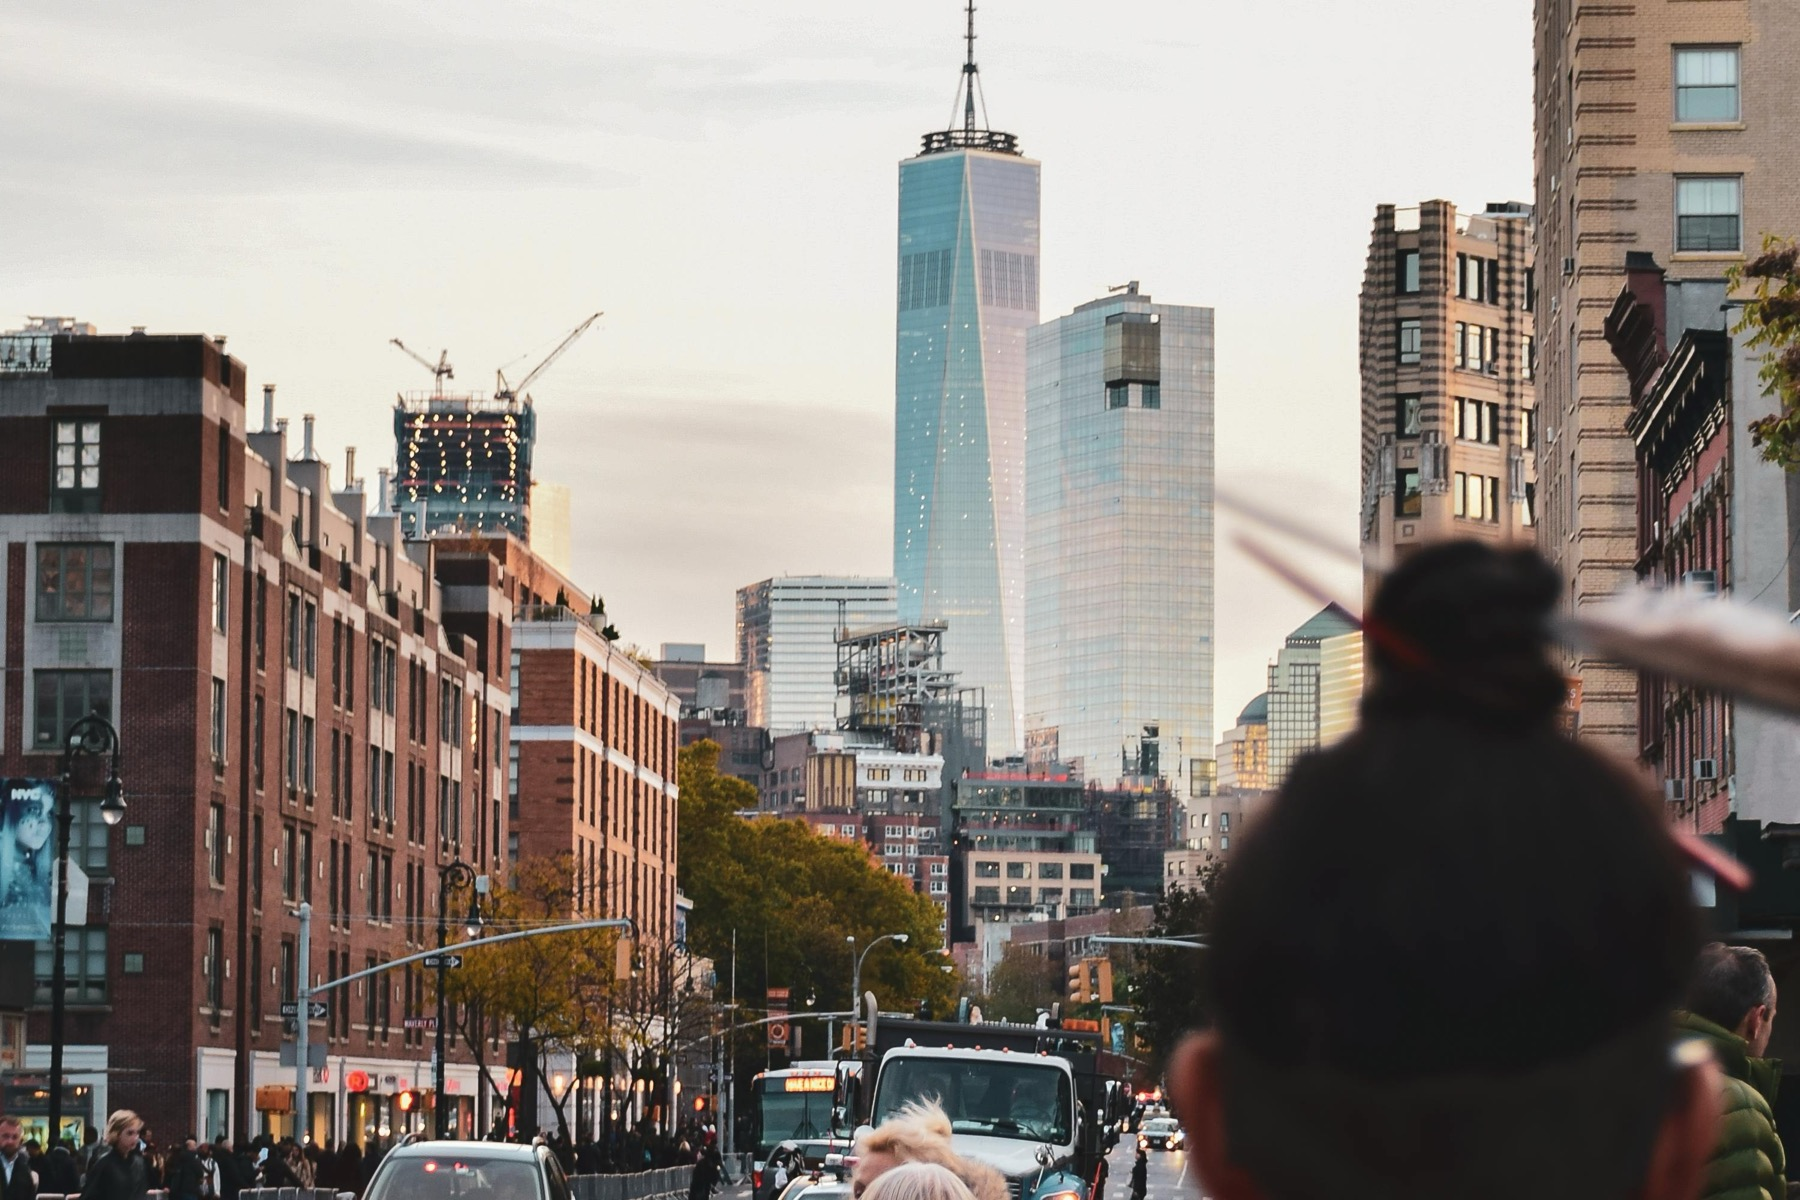
\includegraphics[width=0.25\textwidth]{figures/comparison_on_dataset_A/example_1/input_img.jpg} &

        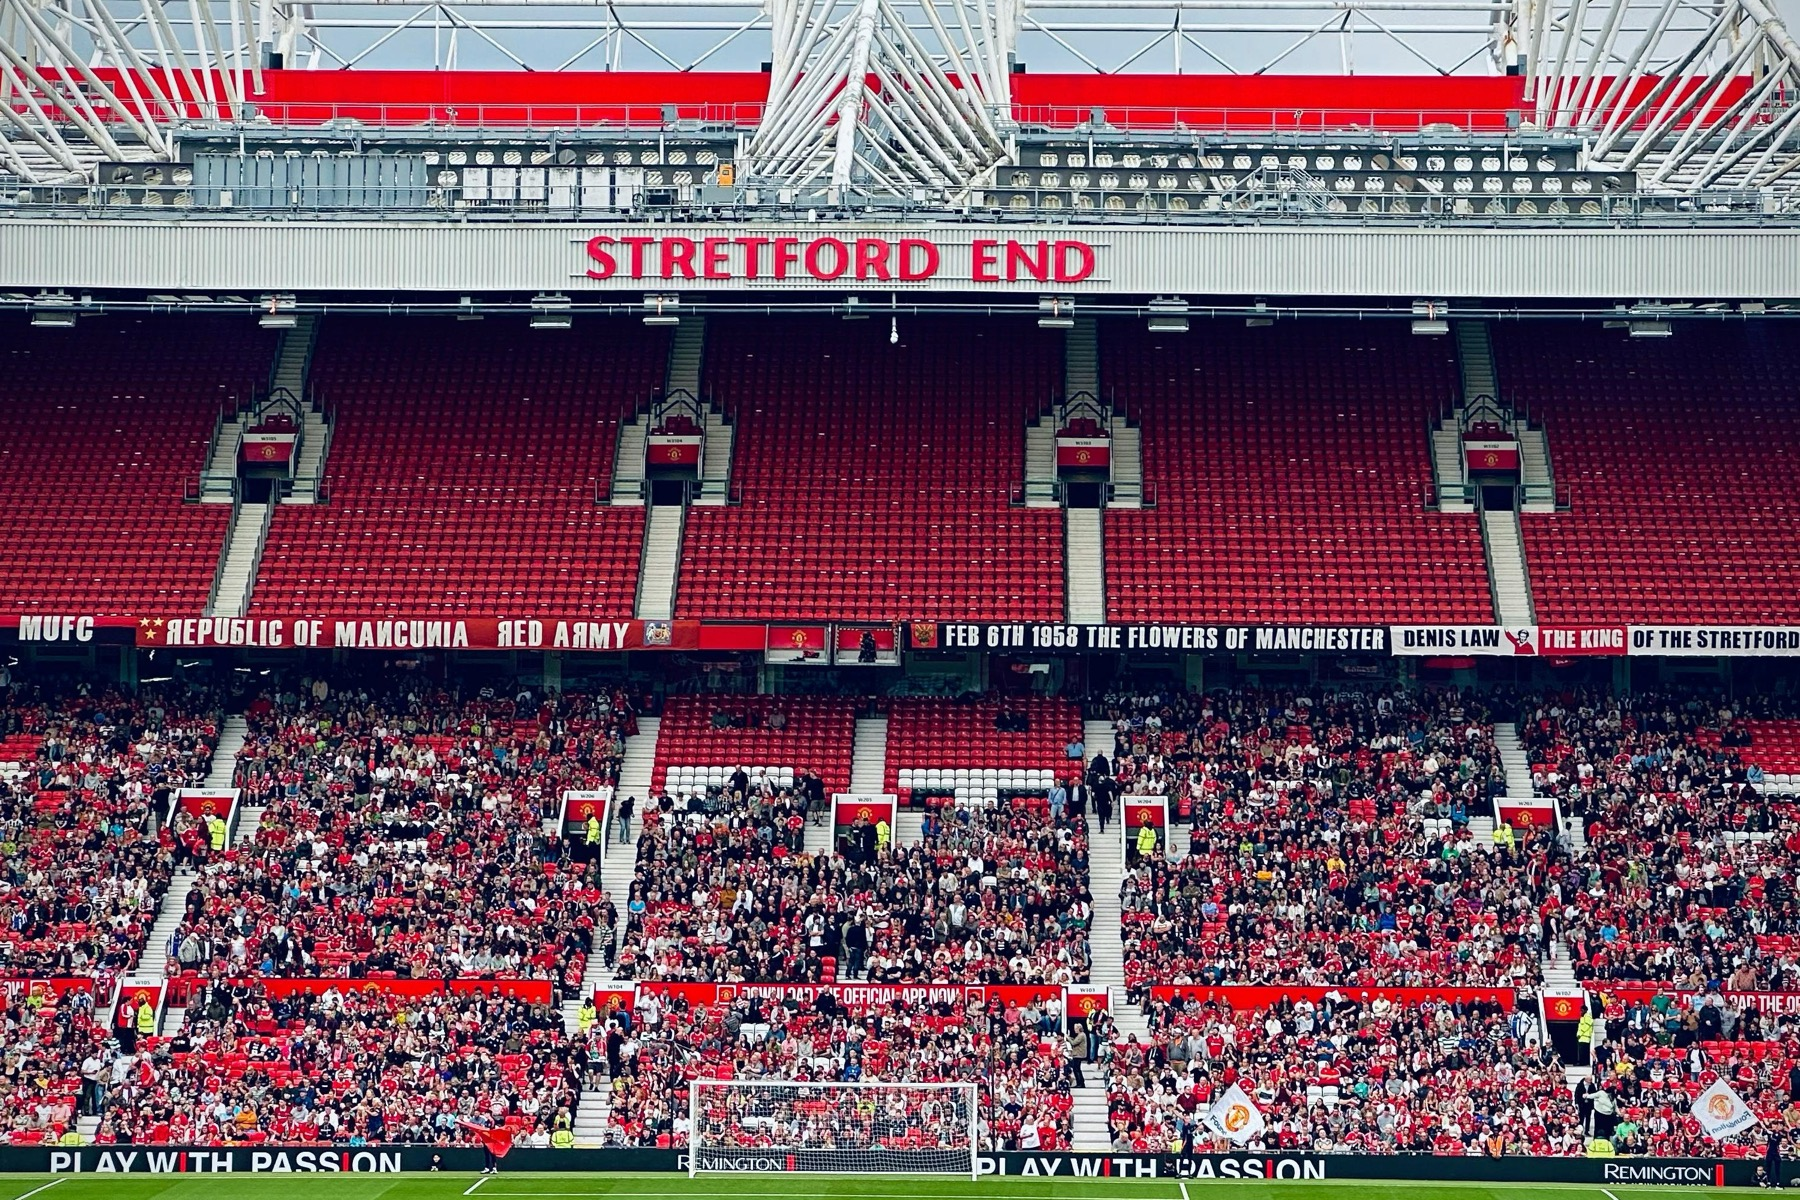
\includegraphics[width=0.25\textwidth]{figures/comparison_on_dataset_A/example_1/method_ResNet.jpg} &

        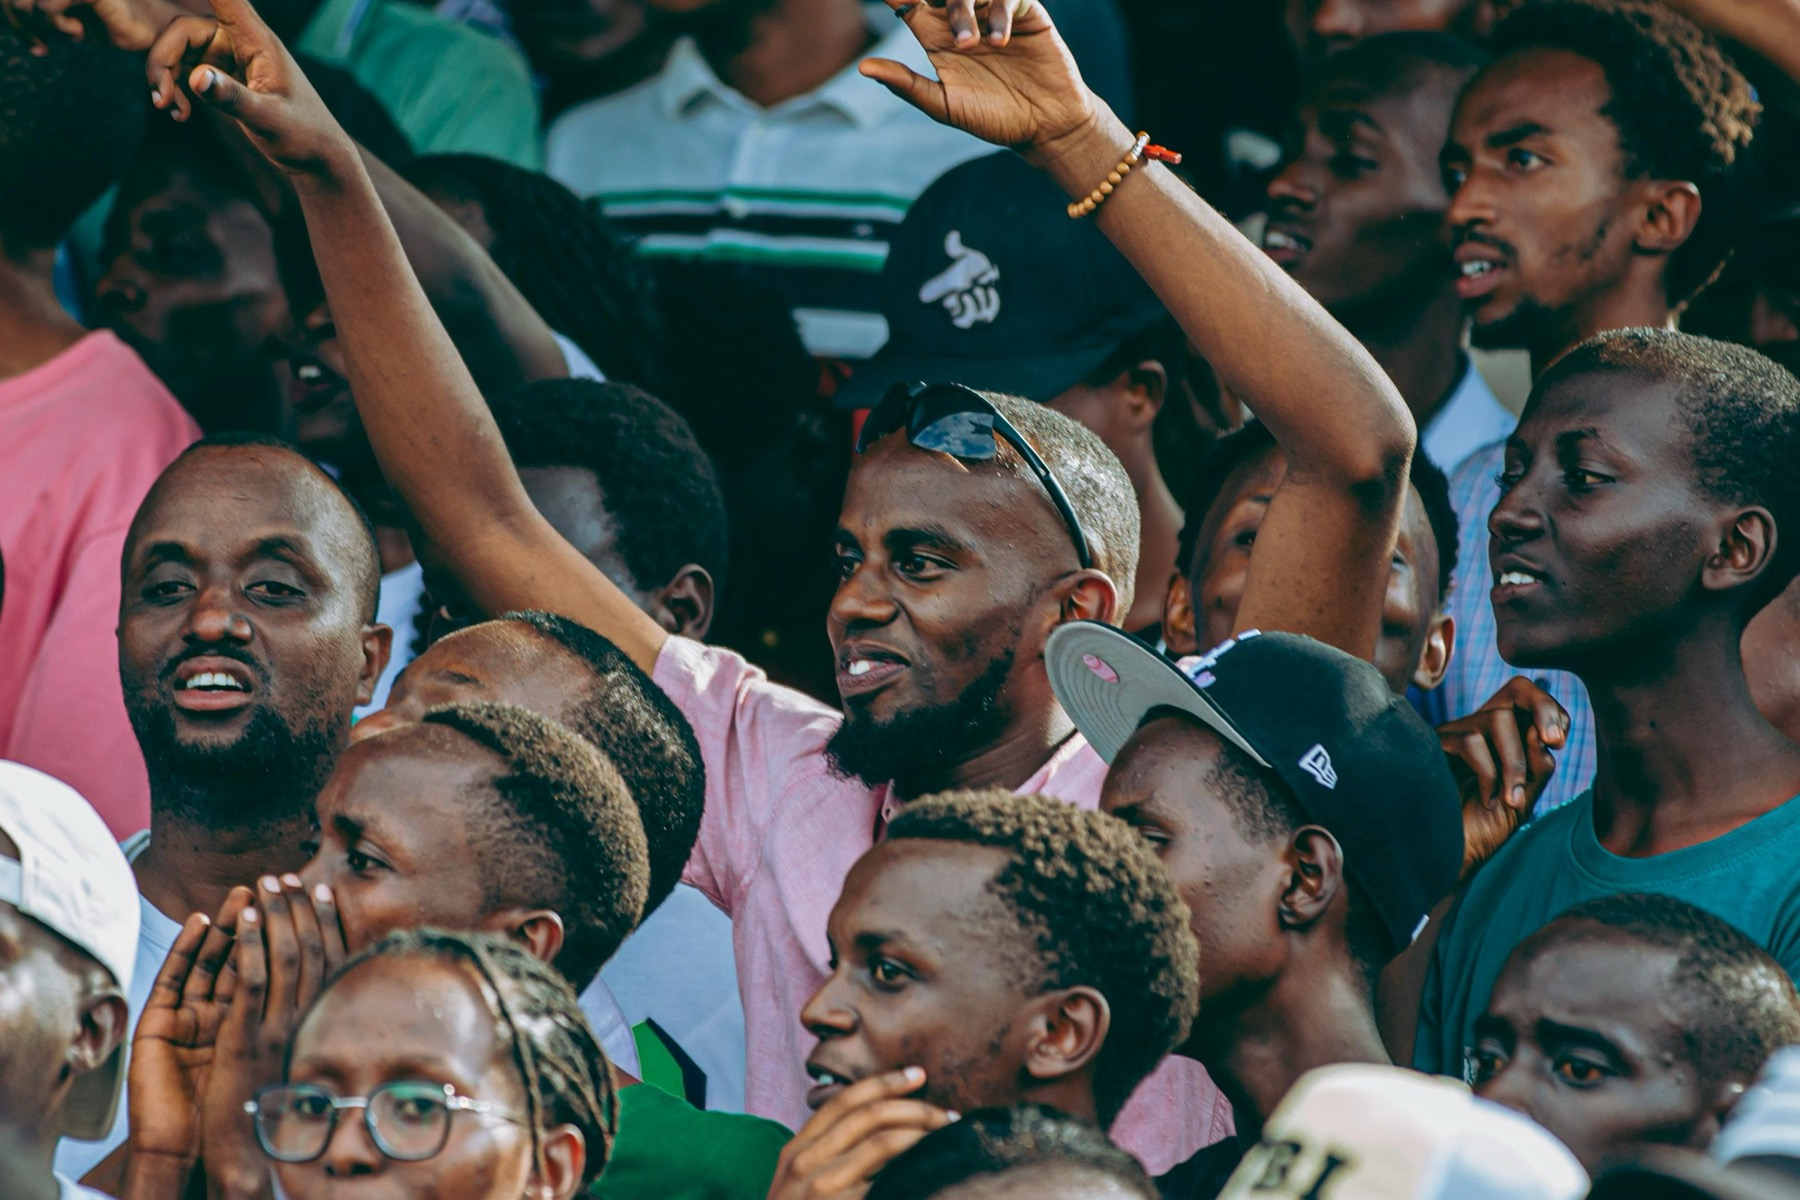
\includegraphics[width=0.25\textwidth]{figures/comparison_on_dataset_A/example_1/method_Transformer.jpg} &

        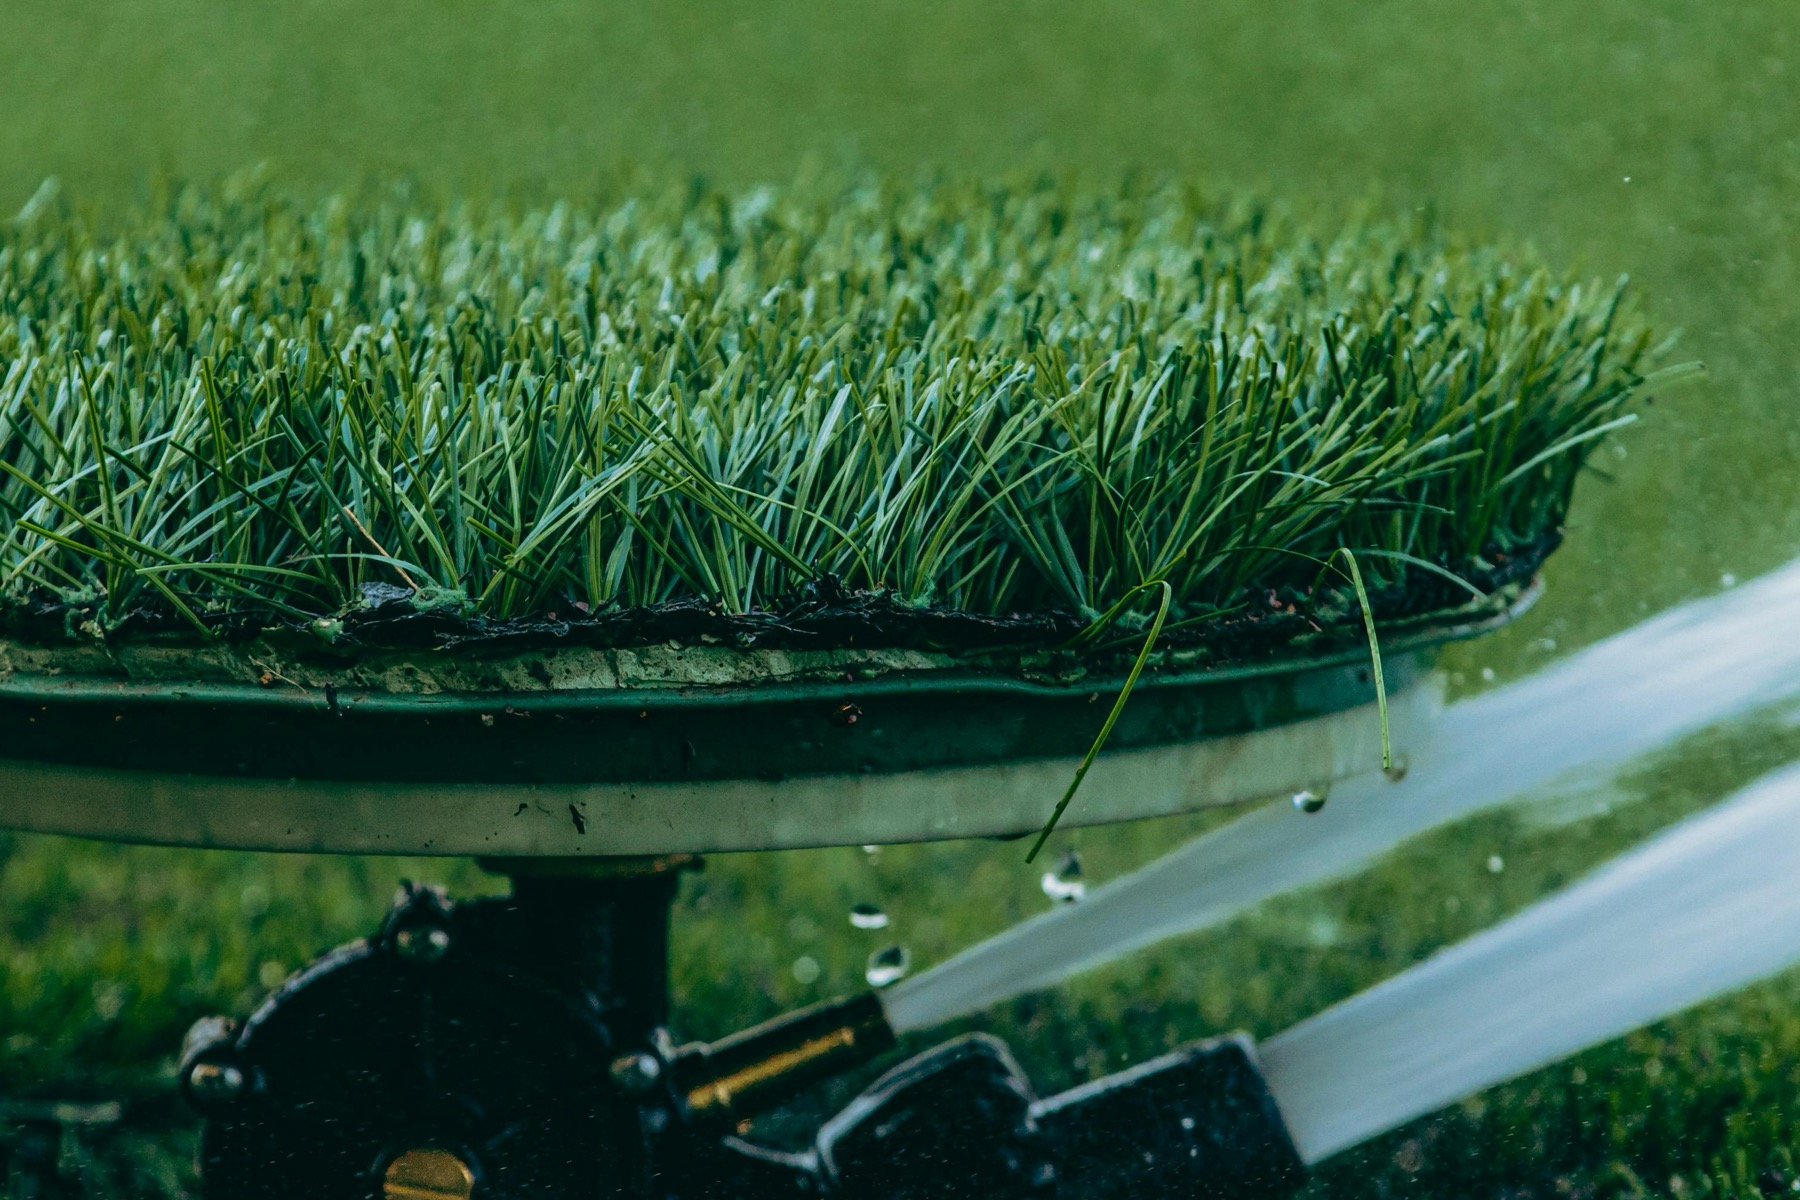
\includegraphics[width=0.25\textwidth]{figures/comparison_on_dataset_A/example_1/method_RNN.jpg} \\

        % 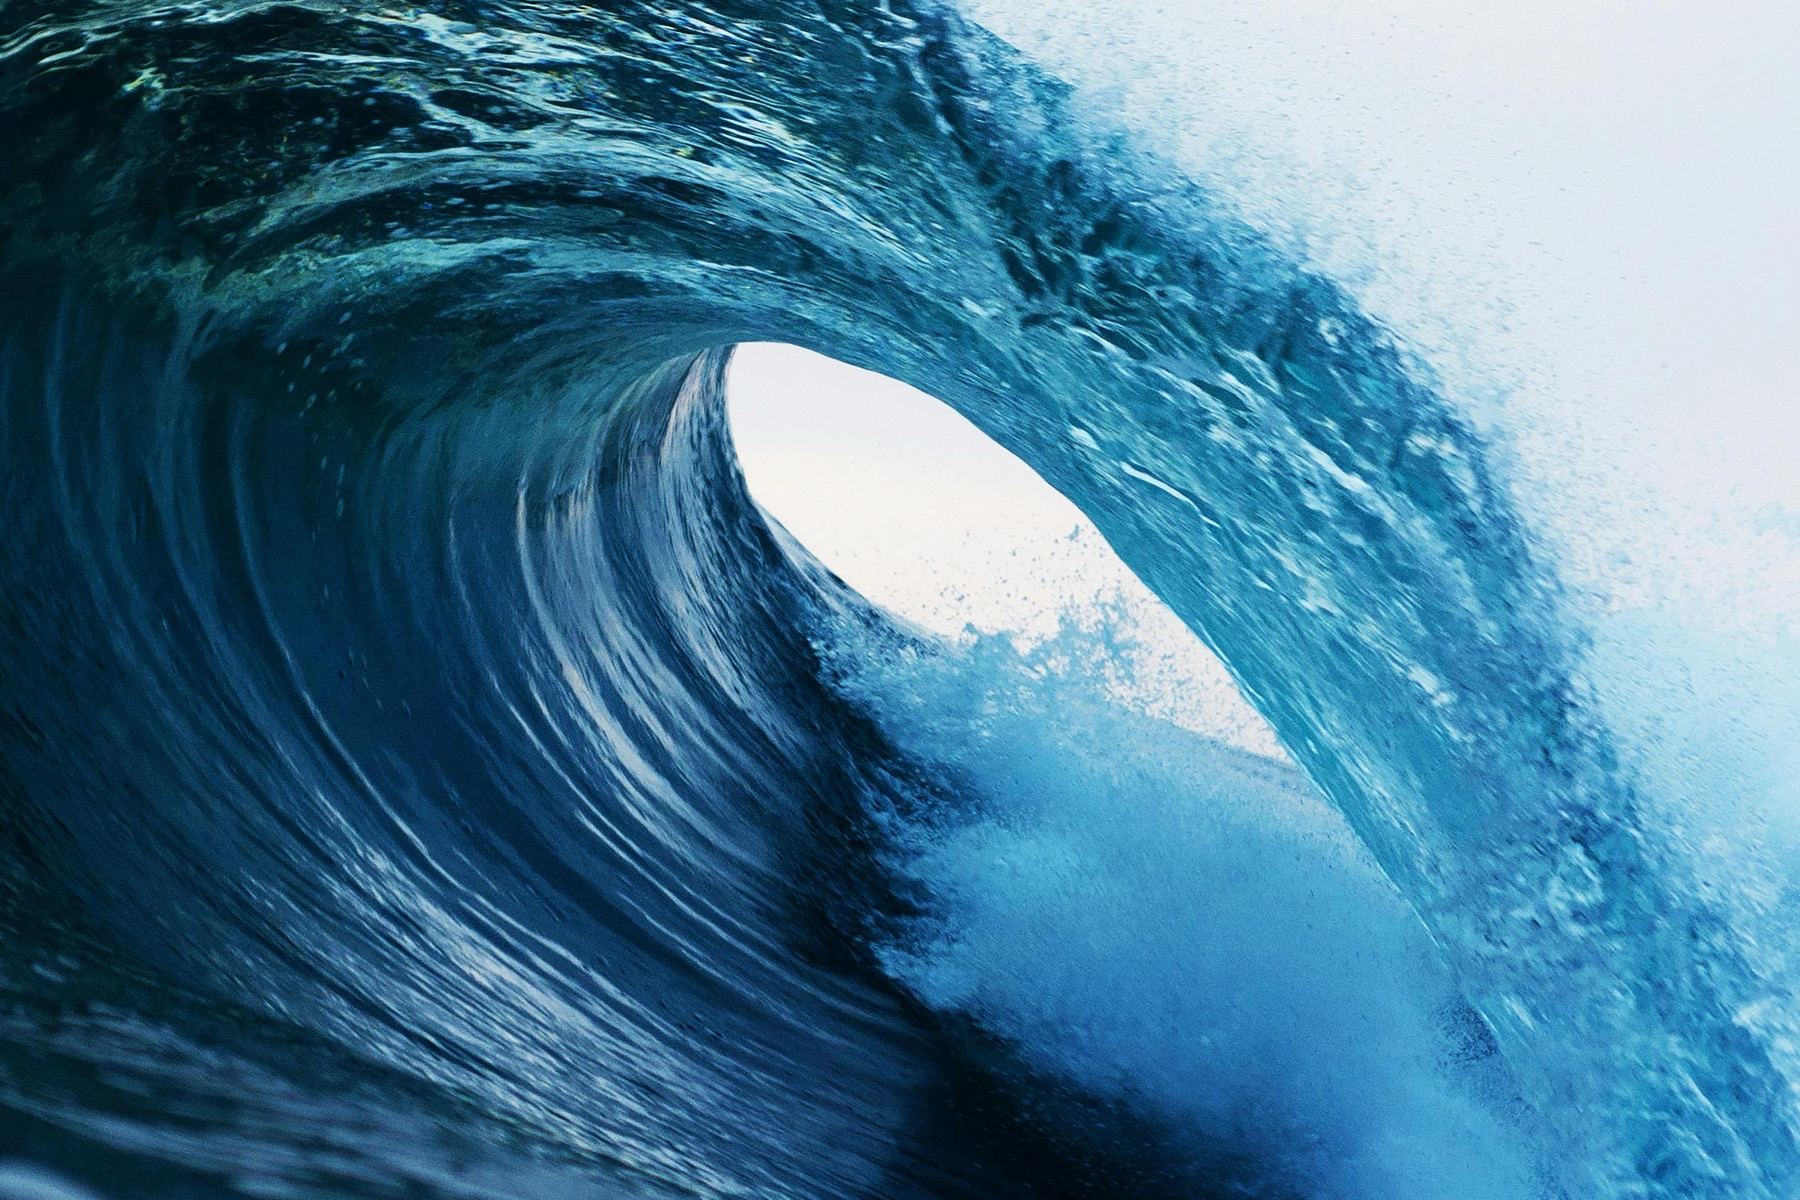
\includegraphics[width=0.25\textwidth]{figures/comparison_on_dataset_A/example_1/method_diffusion.jpg} &

        % 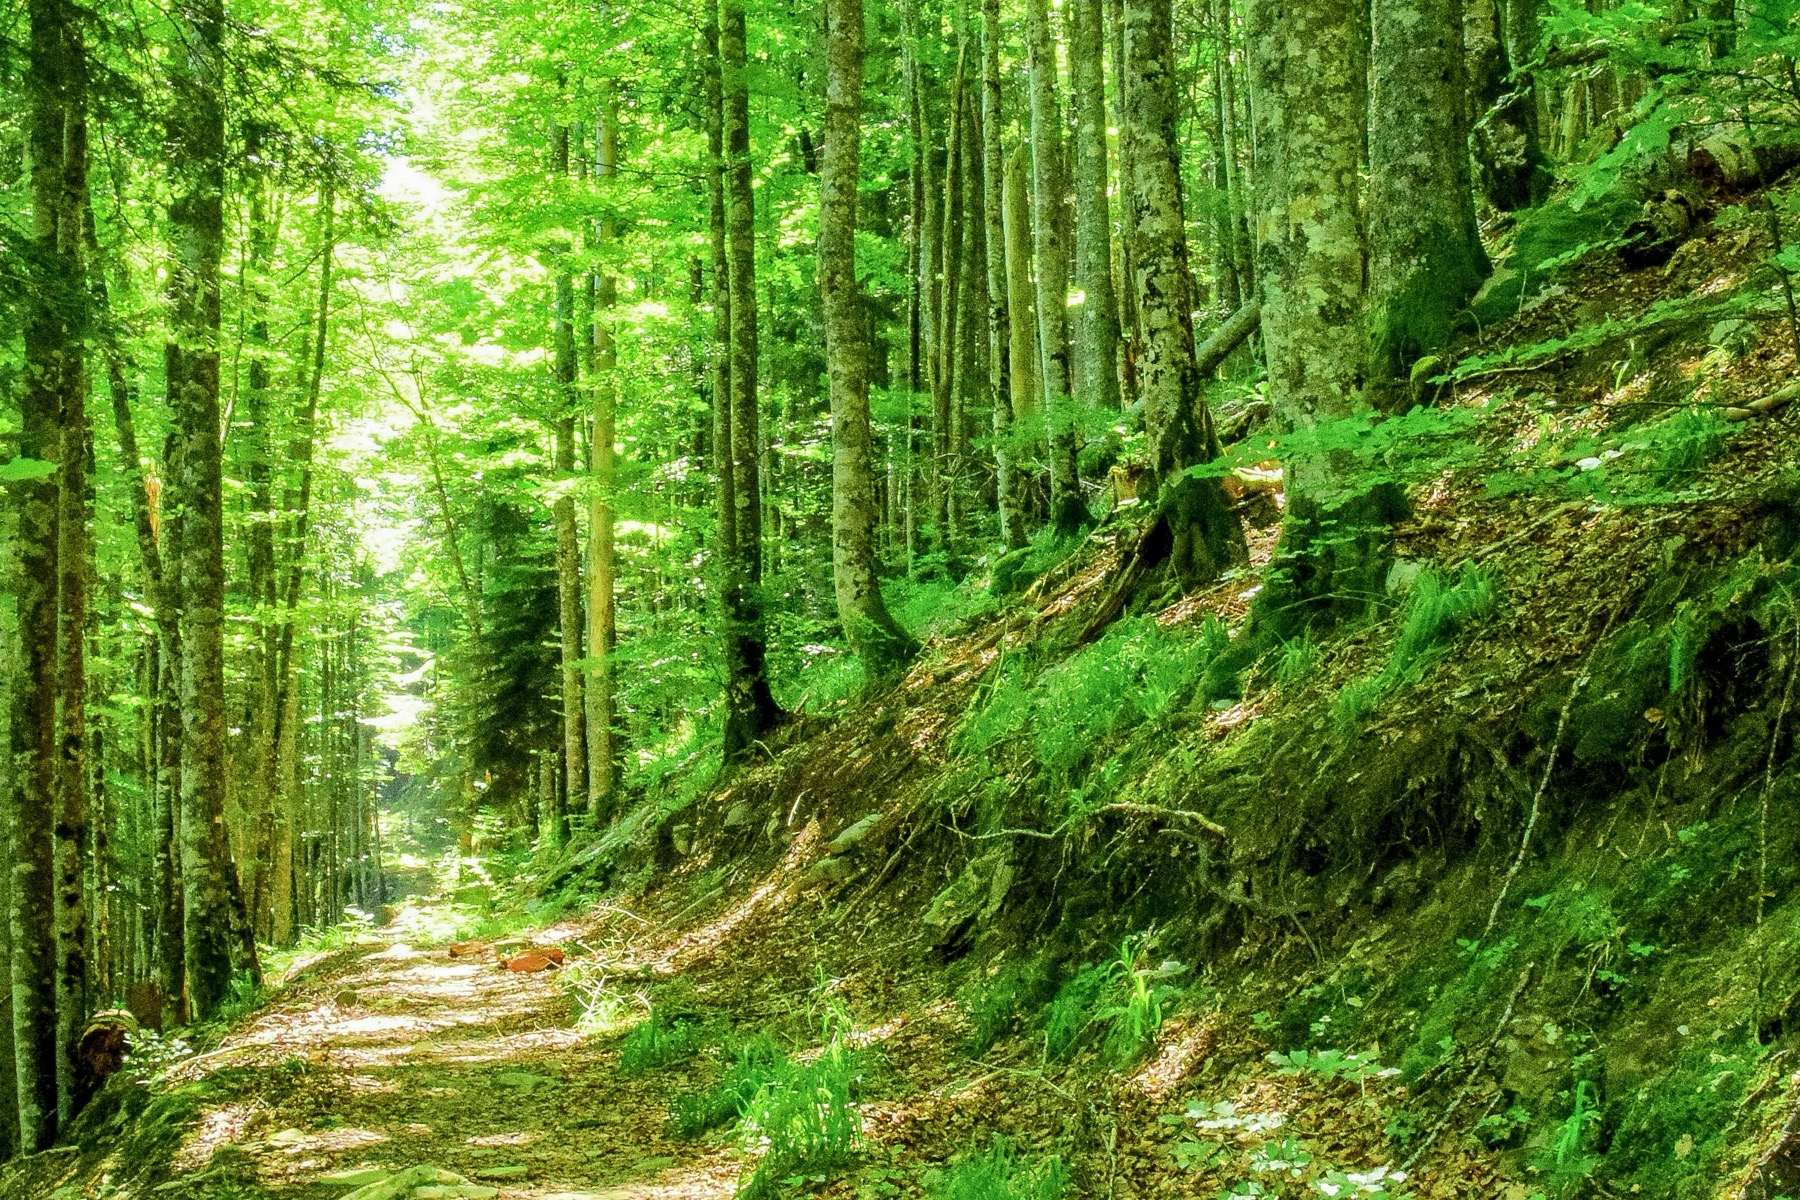
\includegraphics[width=0.25\textwidth]{figures/comparison_on_dataset_A/example_1/method_mamba.jpg} &

        % 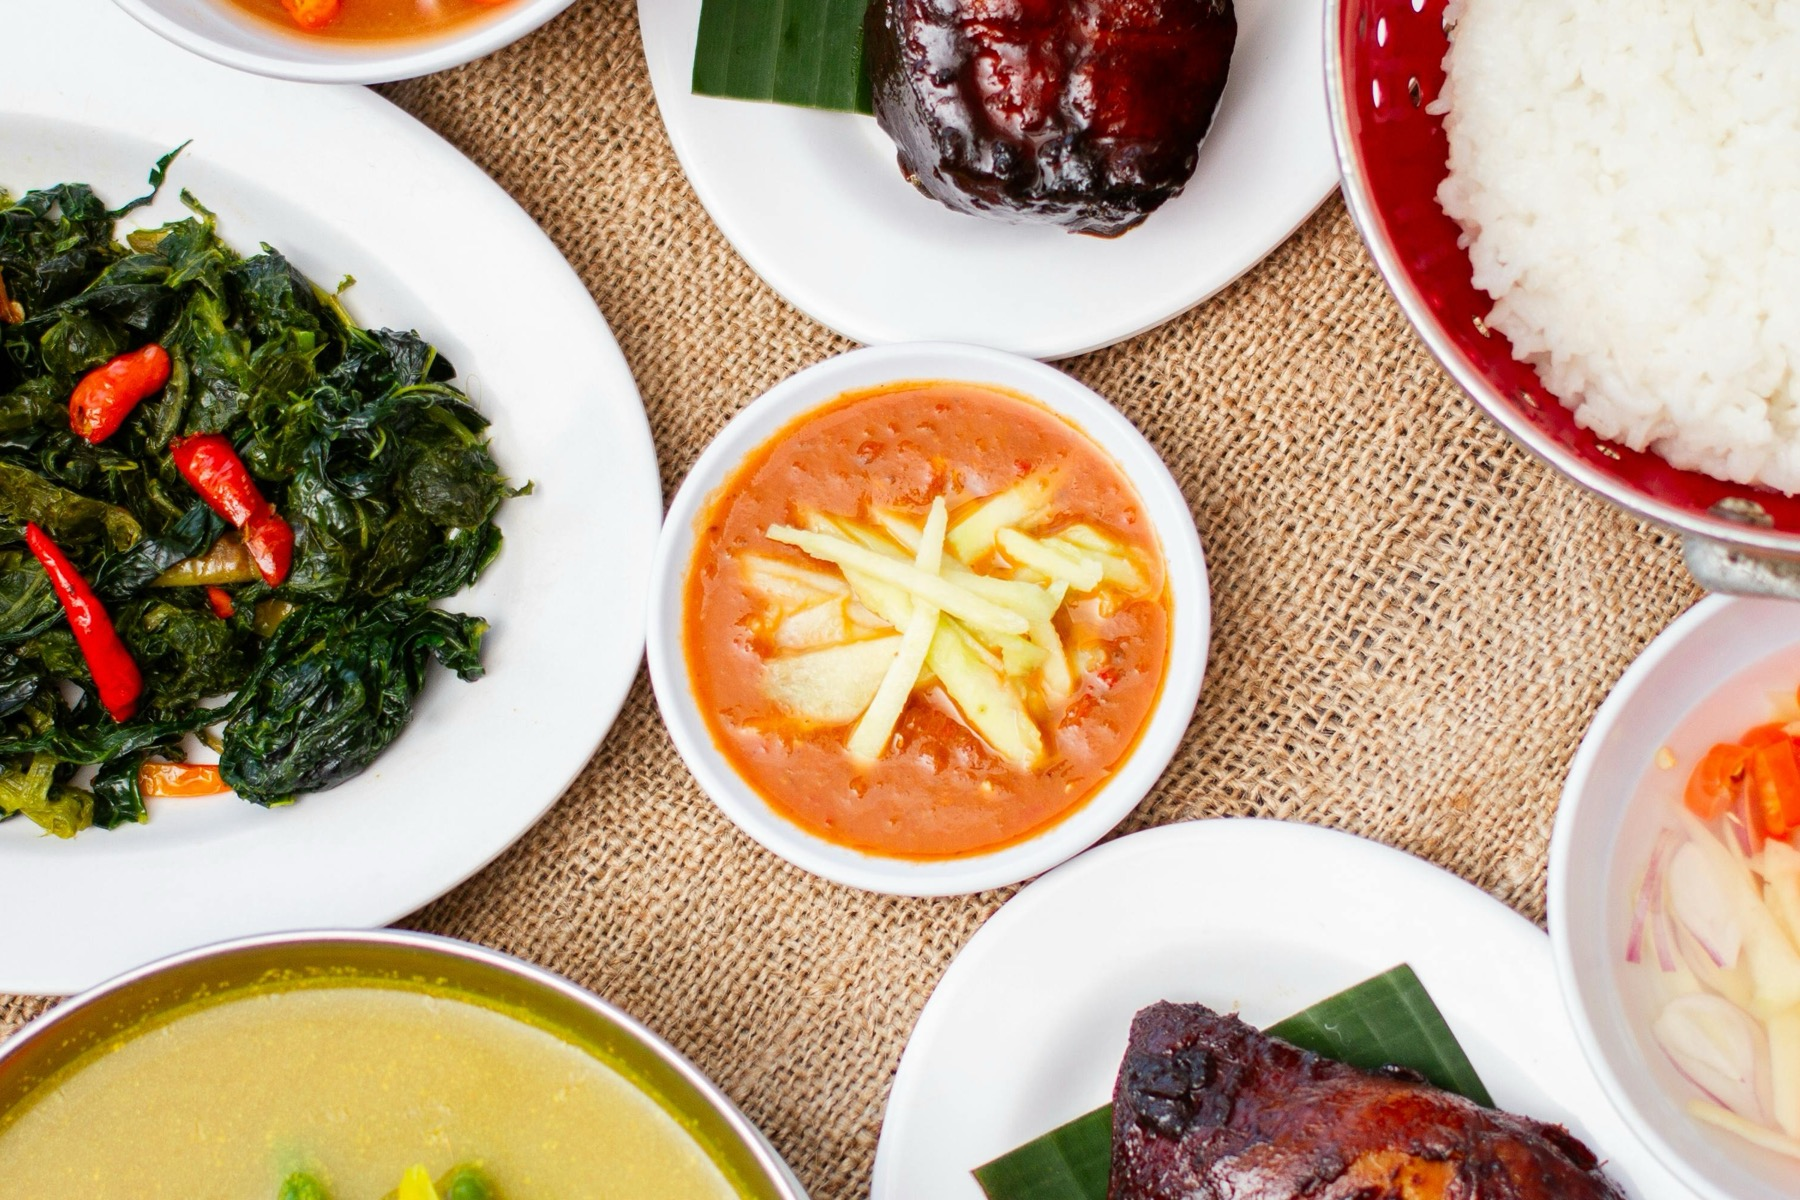
\includegraphics[width=0.25\textwidth]{figures/comparison_on_dataset_A/example_1/method_JEPA.jpg} \\

        
\includegraphics[width=0.25\textwidth]{figures/comparison_on_dataset_A/example_2/input_img.jpg} &

        
\includegraphics[width=0.25\textwidth]{figures/comparison_on_dataset_A/example_2/method_ResNet.jpg} &

        
\includegraphics[width=0.25\textwidth]{figures/comparison_on_dataset_A/example_2/method_Transformer.jpg} &

        
\includegraphics[width=0.25\textwidth]{figures/comparison_on_dataset_A/example_2/method_RNN.jpg} \\

        % 
\includegraphics[width=0.25\textwidth]{figures/comparison_on_dataset_A/example_2/method_diffusion.jpg} &

        % 
\includegraphics[width=0.25\textwidth]{figures/comparison_on_dataset_A/example_2/method_mamba.jpg} &

        % 
\includegraphics[width=0.25\textwidth]{figures/comparison_on_dataset_A/example_2/method_JEPA.jpg} \\

        
\includegraphics[width=0.25\textwidth]{figures/comparison_on_dataset_A/example_5/input_img.jpg} &

        
\includegraphics[width=0.25\textwidth]{figures/comparison_on_dataset_A/example_5/method_ResNet.jpg} &

        
\includegraphics[width=0.25\textwidth]{figures/comparison_on_dataset_A/example_5/method_Transformer.jpg} &

        
\includegraphics[width=0.25\textwidth]{figures/comparison_on_dataset_A/example_5/method_RNN.jpg}

        % 
\includegraphics[width=0.25\textwidth]{figures/comparison_on_dataset_A/example_5/method_diffusion.jpg} &

        % 
\includegraphics[width=0.25\textwidth]{figures/comparison_on_dataset_A/example_5/method_mamba.jpg} &

        % 
\includegraphics[width=0.25\textwidth]{figures/comparison_on_dataset_A/example_5/method_JEPA.jpg}

    \end{tabular}

    \caption{Qualitative comparison on Dataset A. Each row shows one example, and each column shows the input image or the result from a different method. 
    }

    \label{fig:comparison_dataset_A}

\end{figure*}


\begin{figure*}[t]

    \centering

    \setlength{\tabcolsep}{2pt}

    \renewcommand{\arraystretch}{0.8}

    \begin{tabular}{cccc}

        \textbf{Input} & \textbf{Diffusion} & \textbf{Mamba} & \textbf{JEPA} \\

        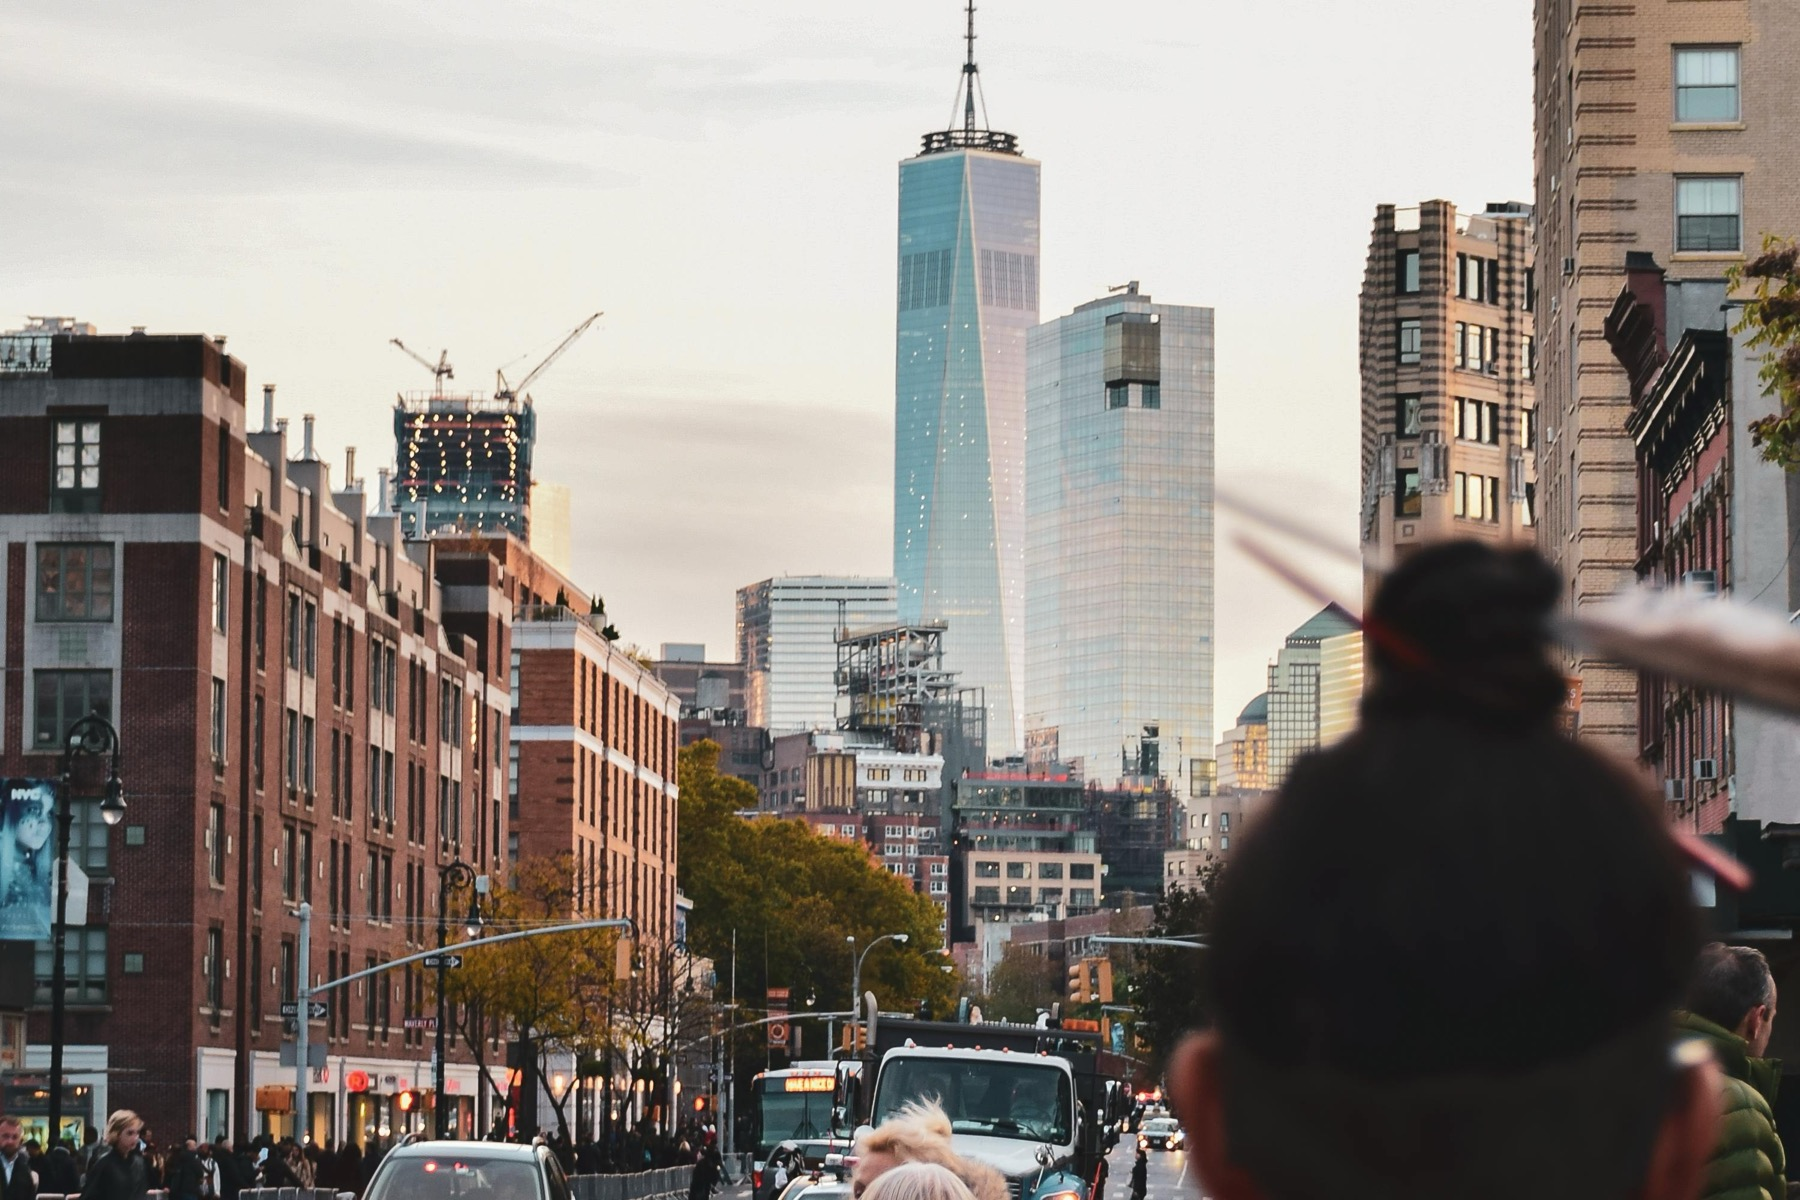
\includegraphics[width=0.25\textwidth]{figures/comparison_on_dataset_A/example_1/input_img.jpg} &

        % 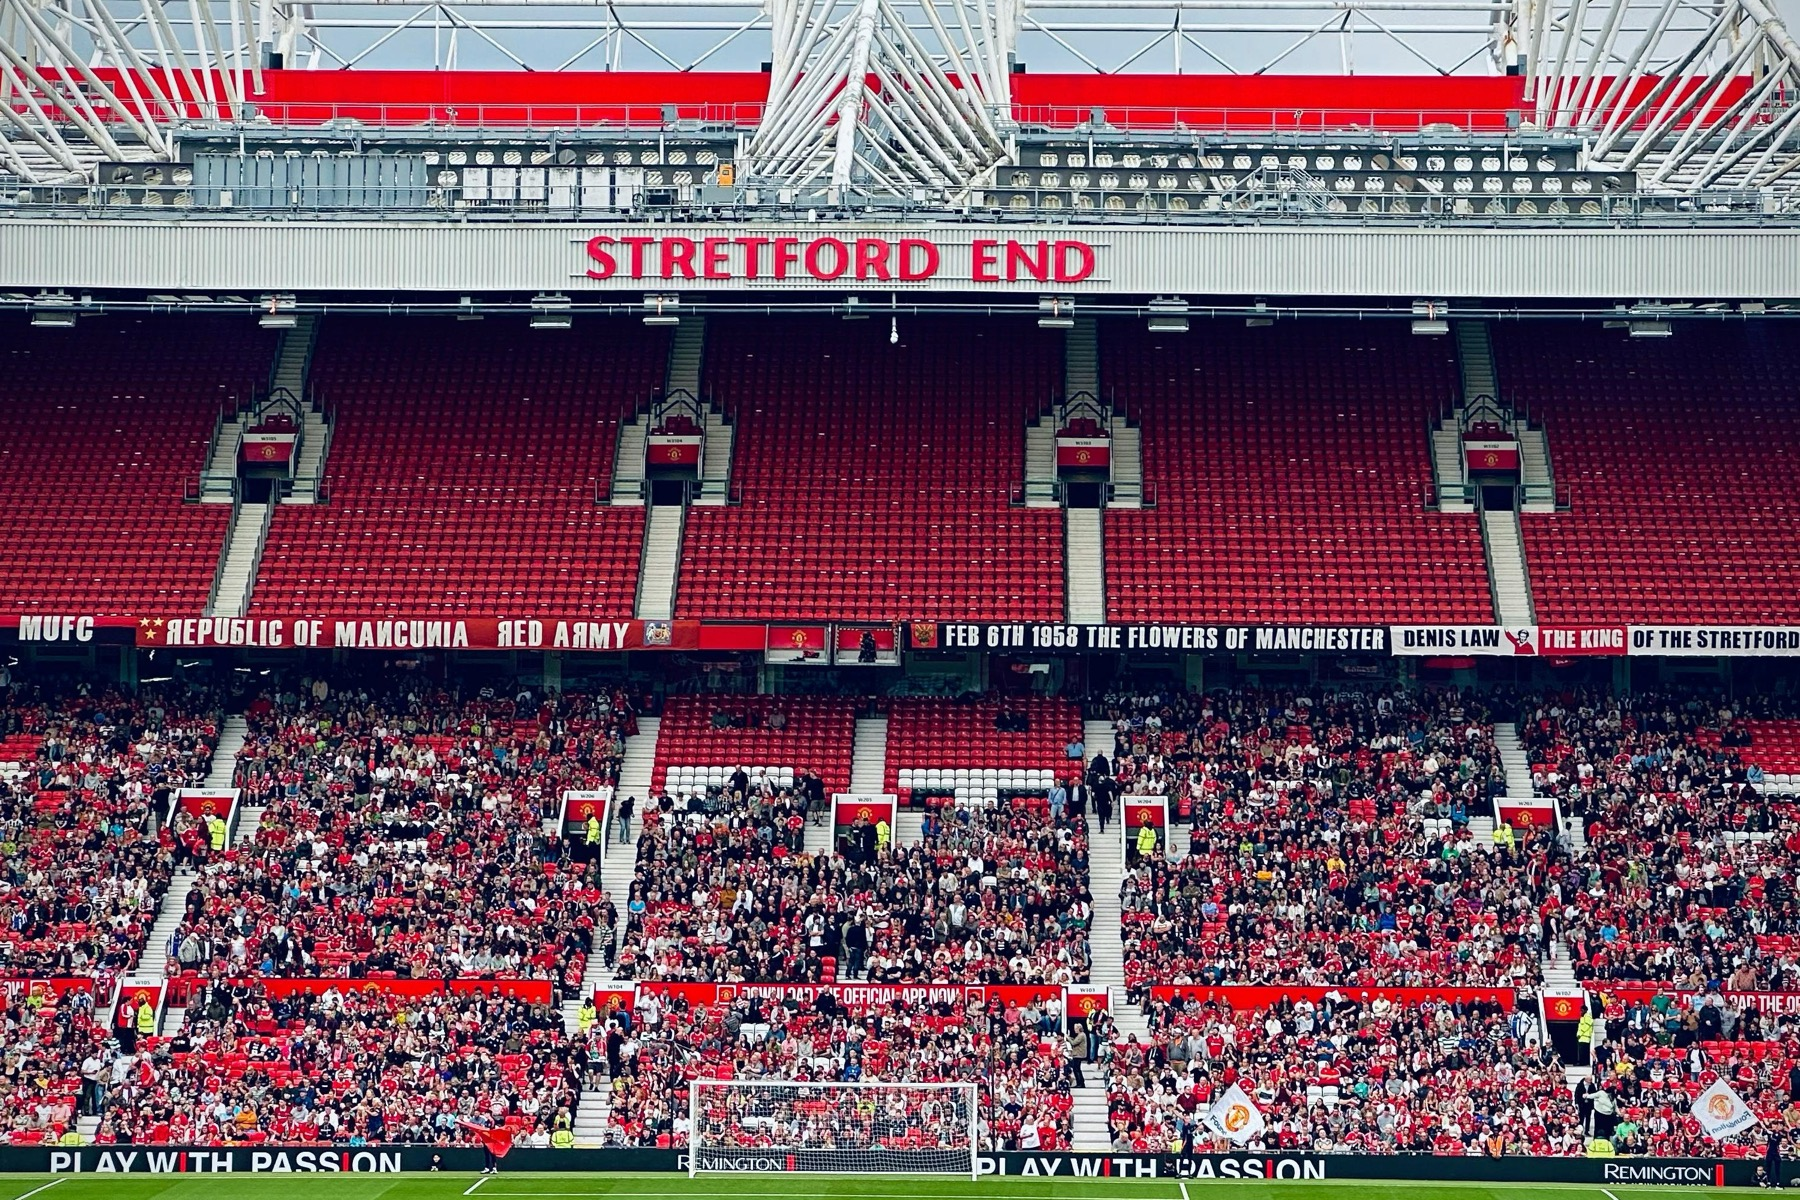
\includegraphics[width=0.25\textwidth]{figures/comparison_on_dataset_A/example_1/method_ResNet.jpg} &

        % 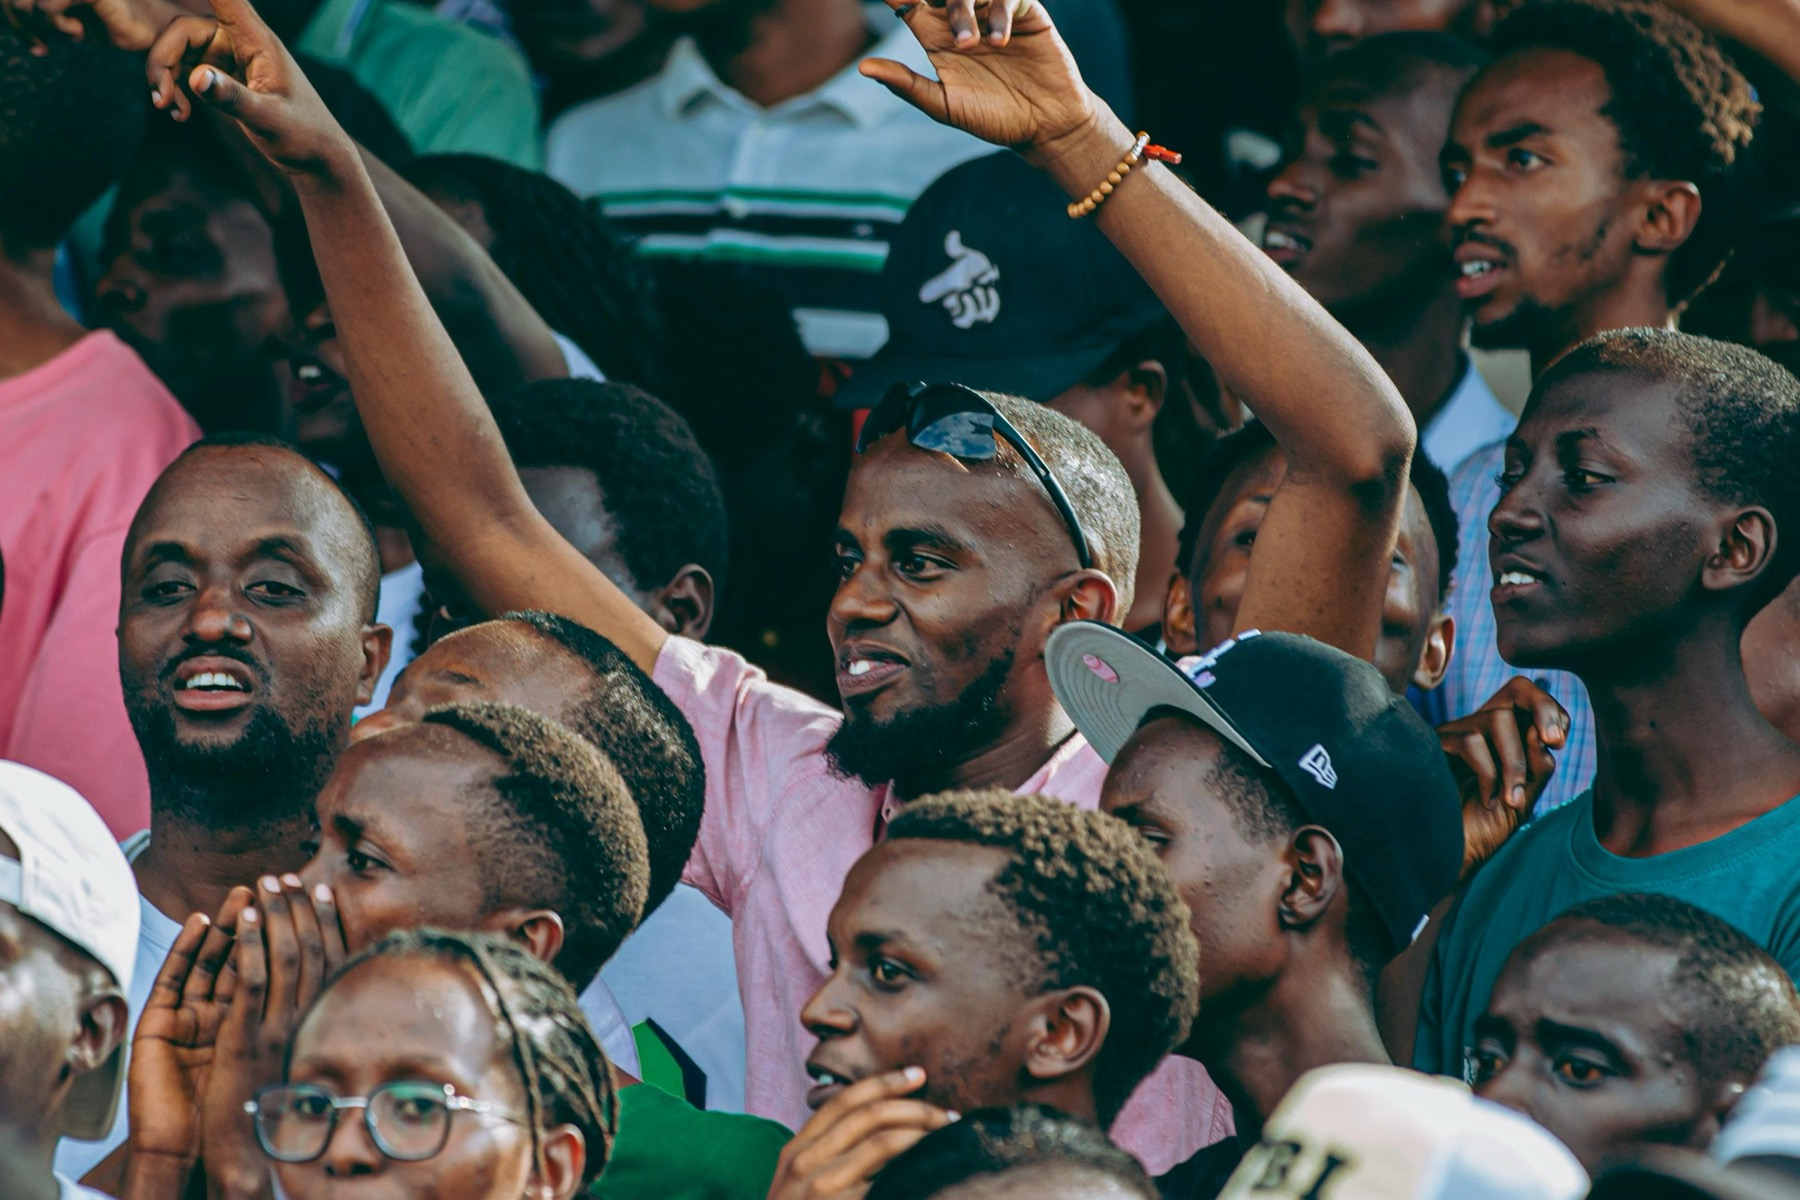
\includegraphics[width=0.25\textwidth]{figures/comparison_on_dataset_A/example_1/method_Transformer.jpg} &

        % 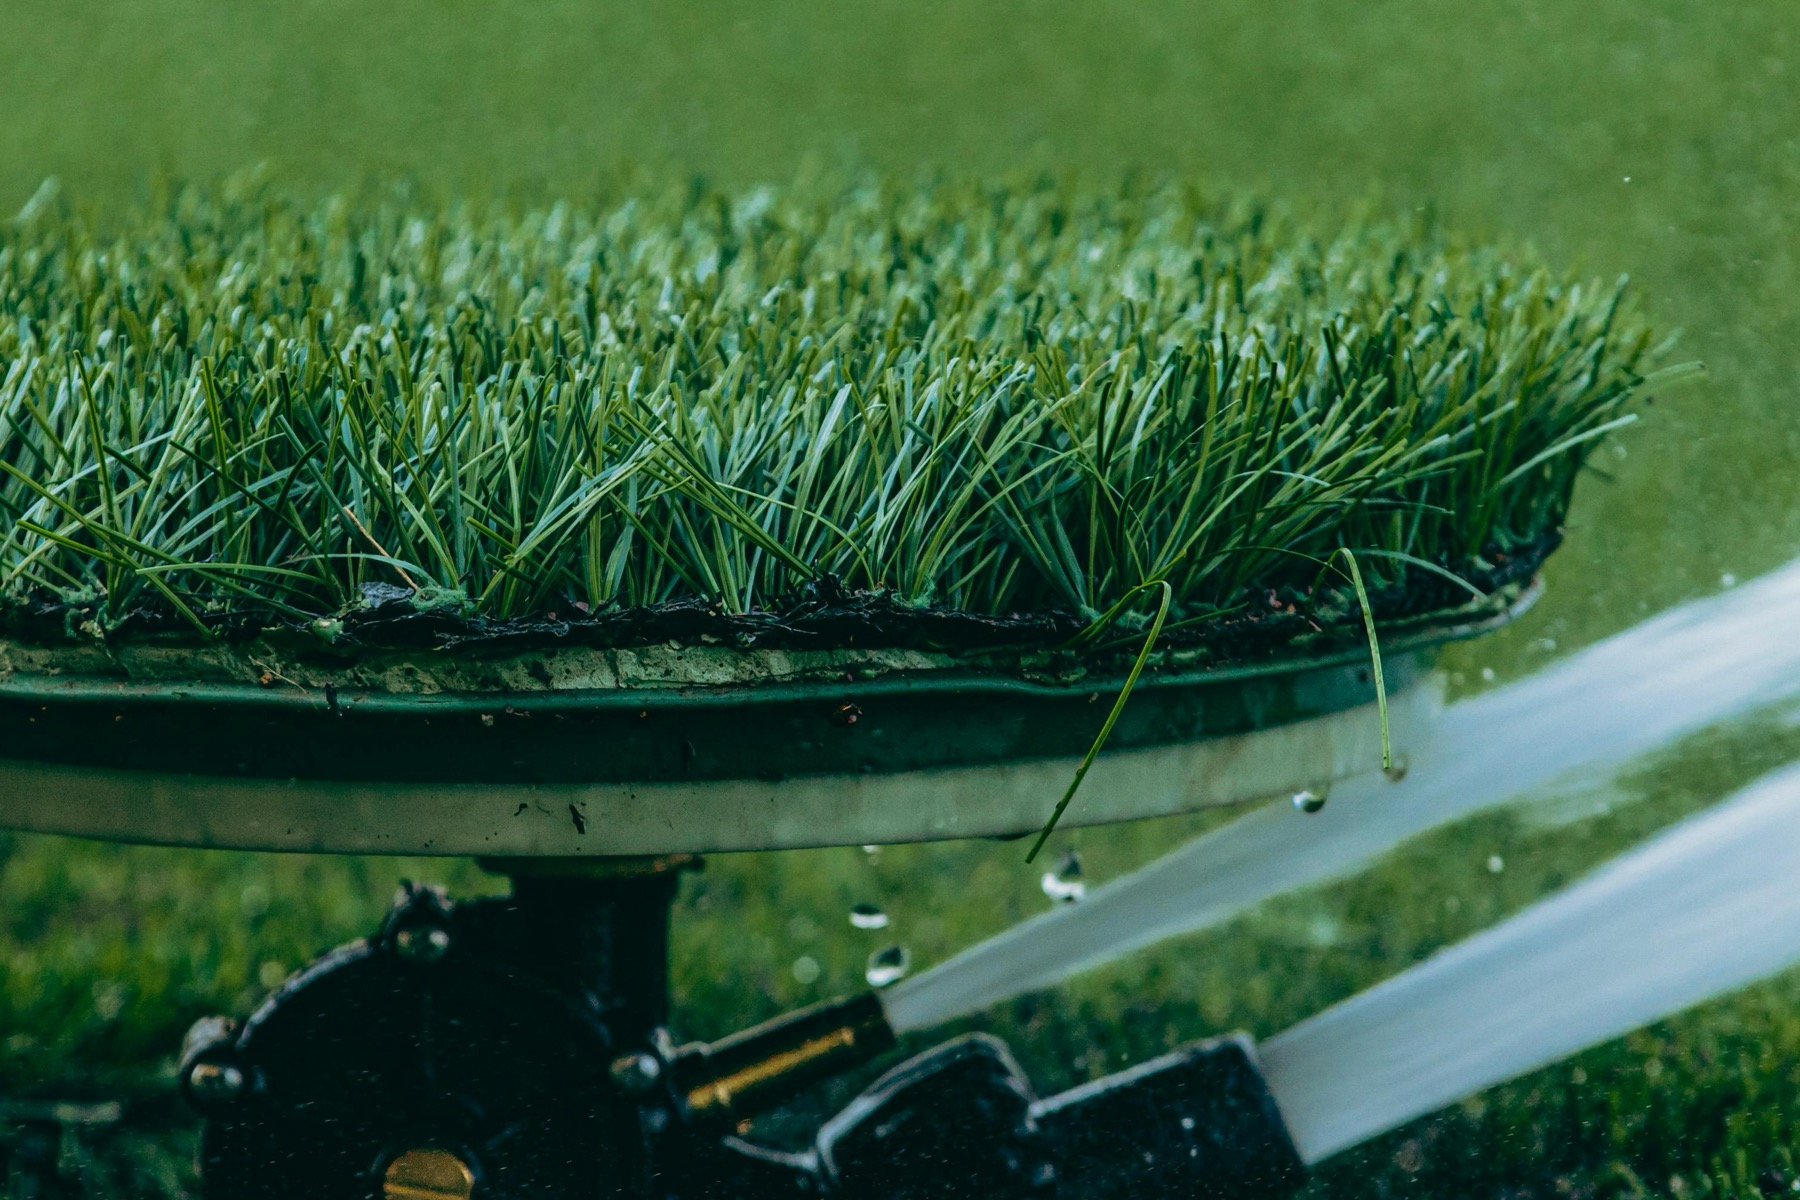
\includegraphics[width=0.25\textwidth]{figures/comparison_on_dataset_A/example_1/method_RNN.jpg} &

        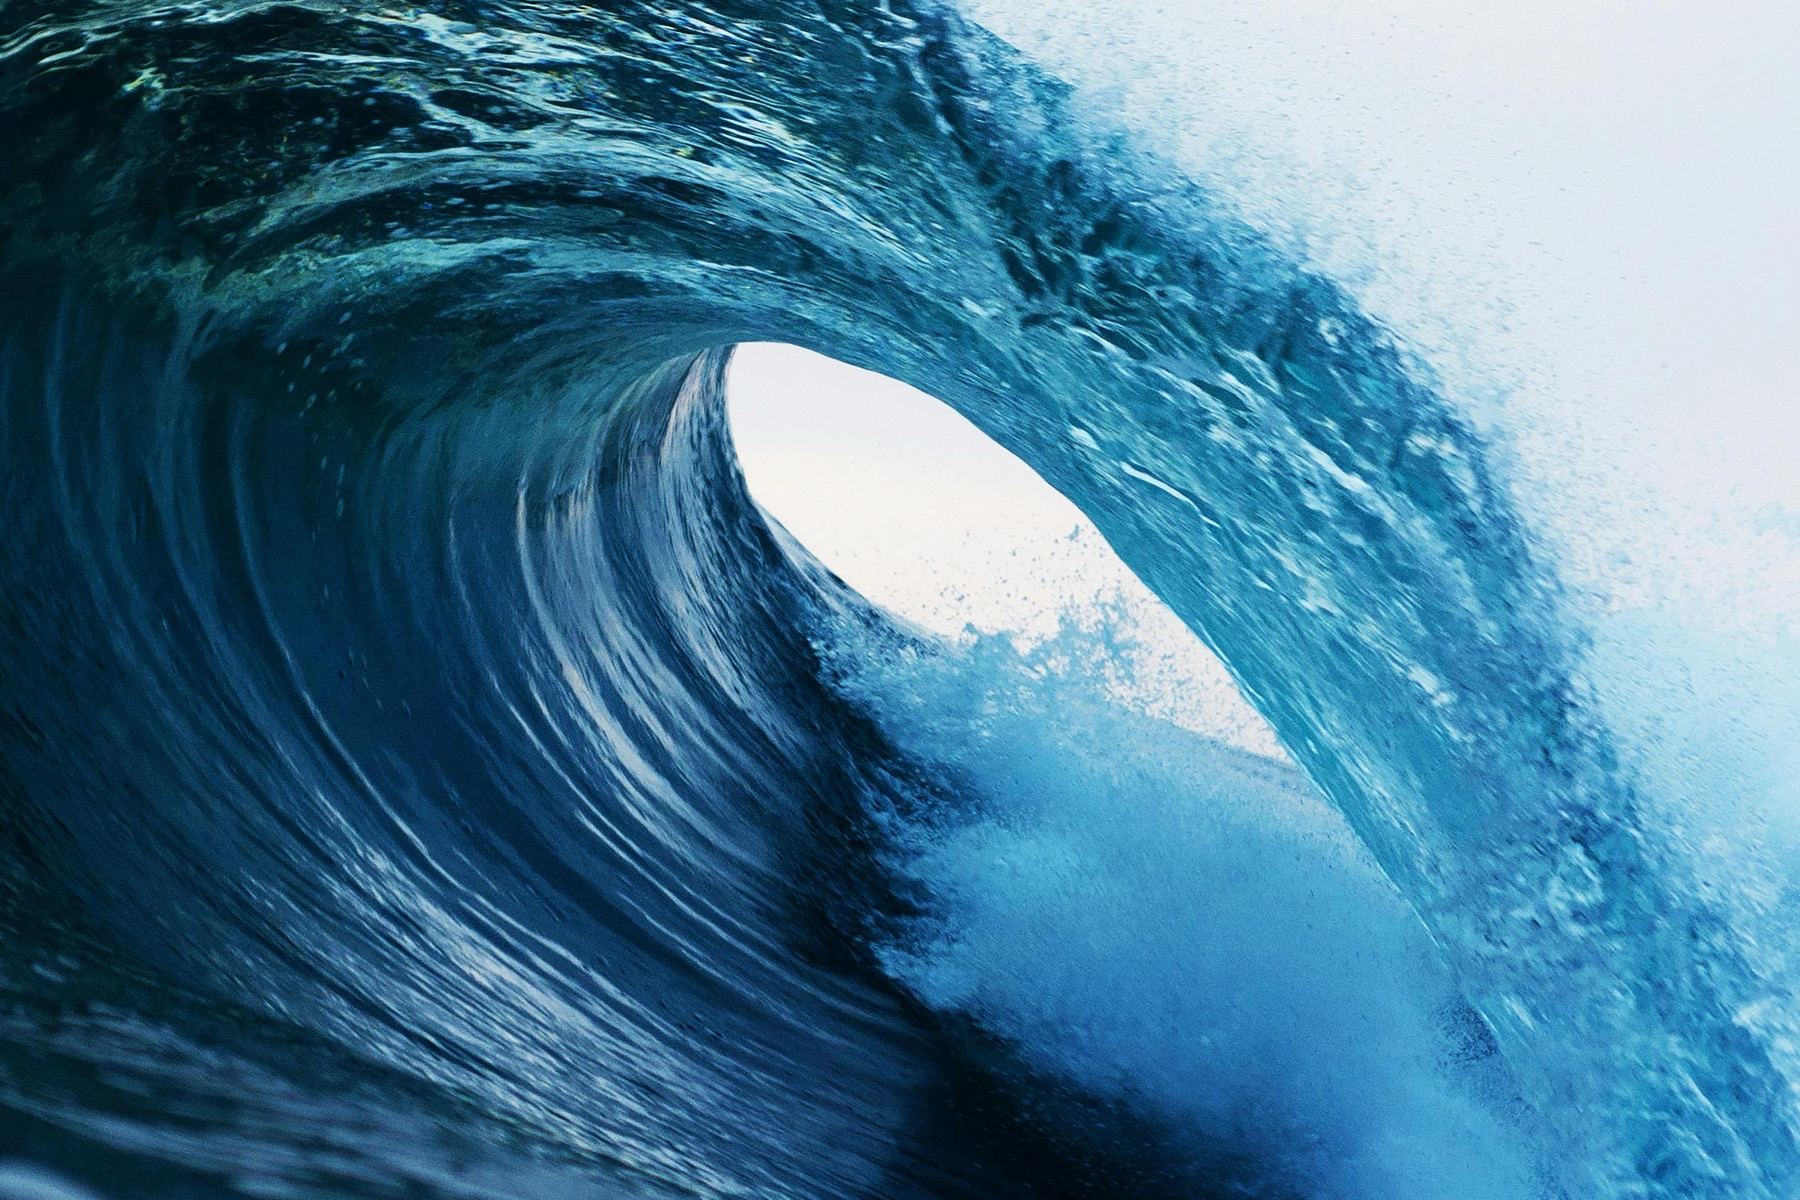
\includegraphics[width=0.25\textwidth]{figures/comparison_on_dataset_A/example_1/method_diffusion.jpg} &

        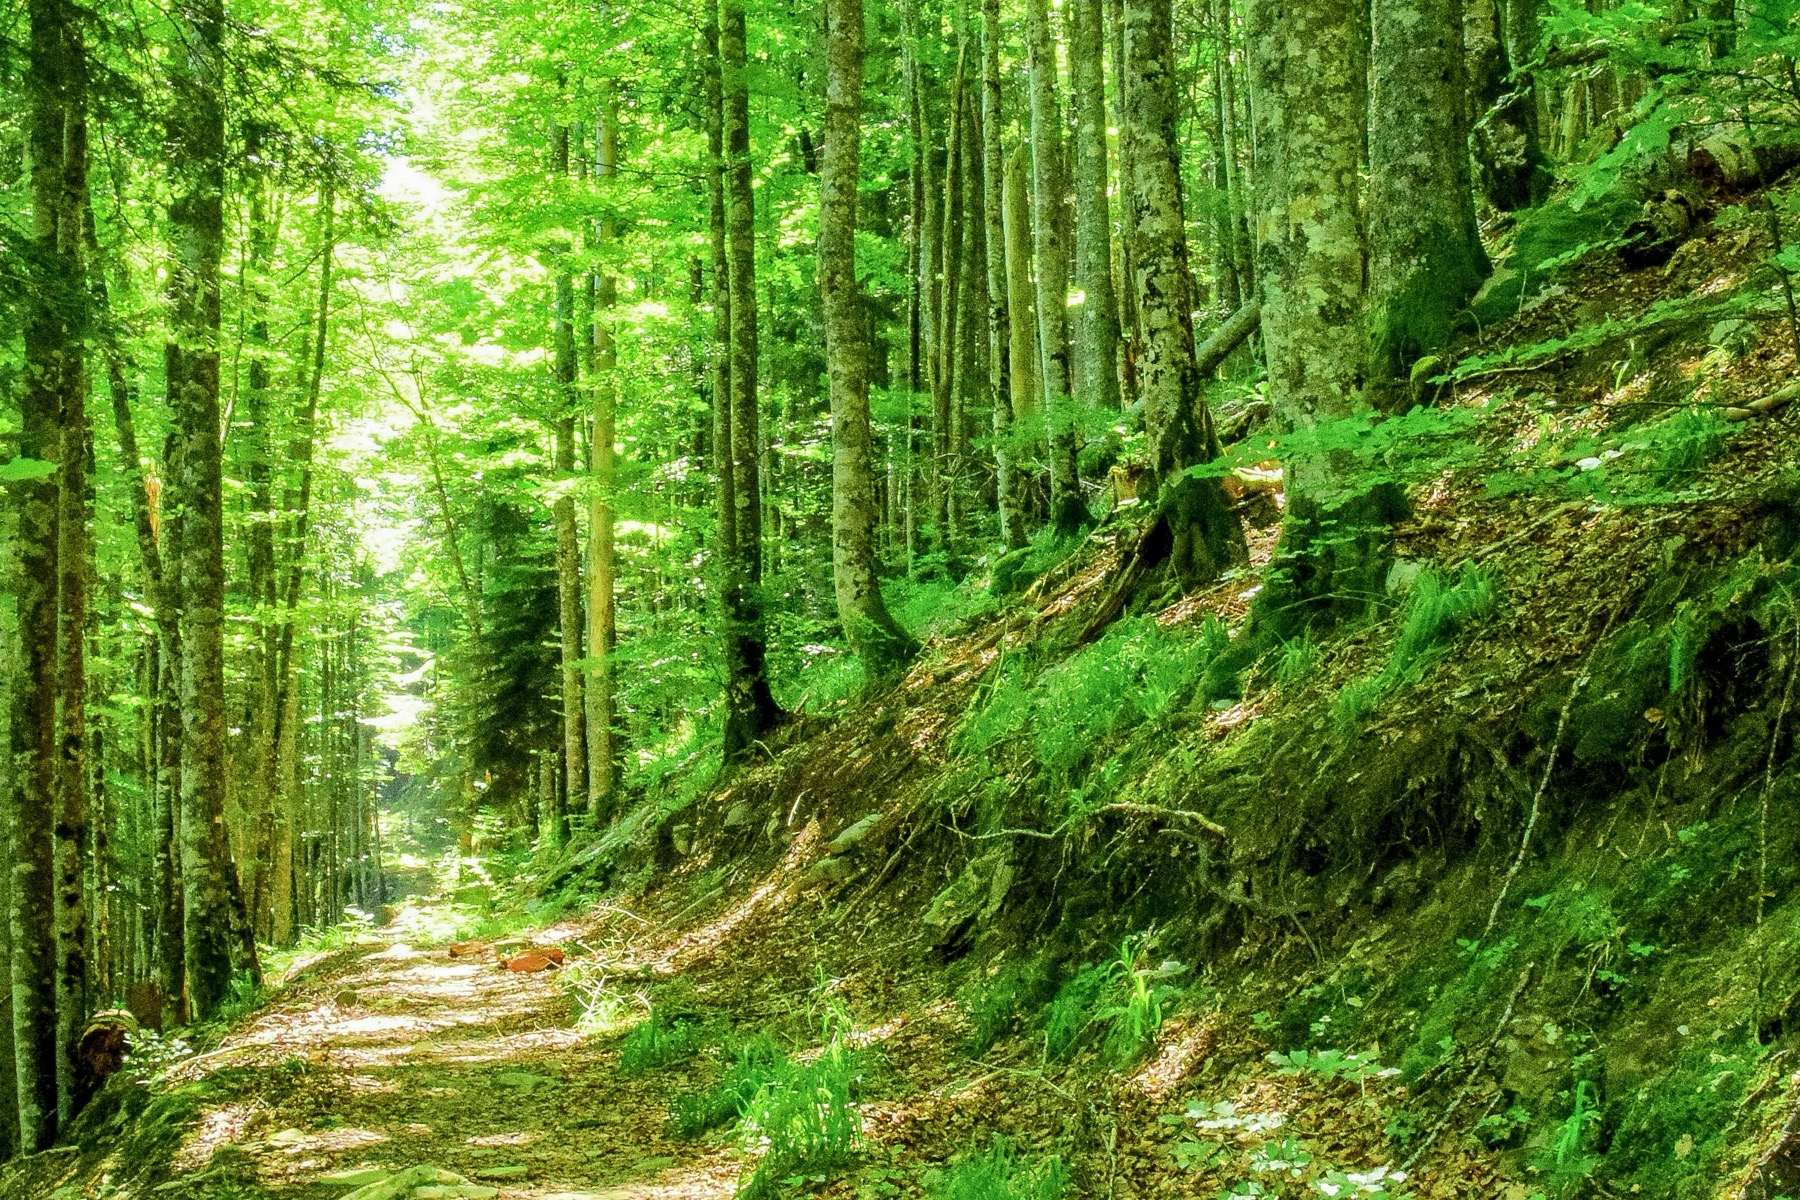
\includegraphics[width=0.25\textwidth]{figures/comparison_on_dataset_A/example_1/method_mamba.jpg} &

        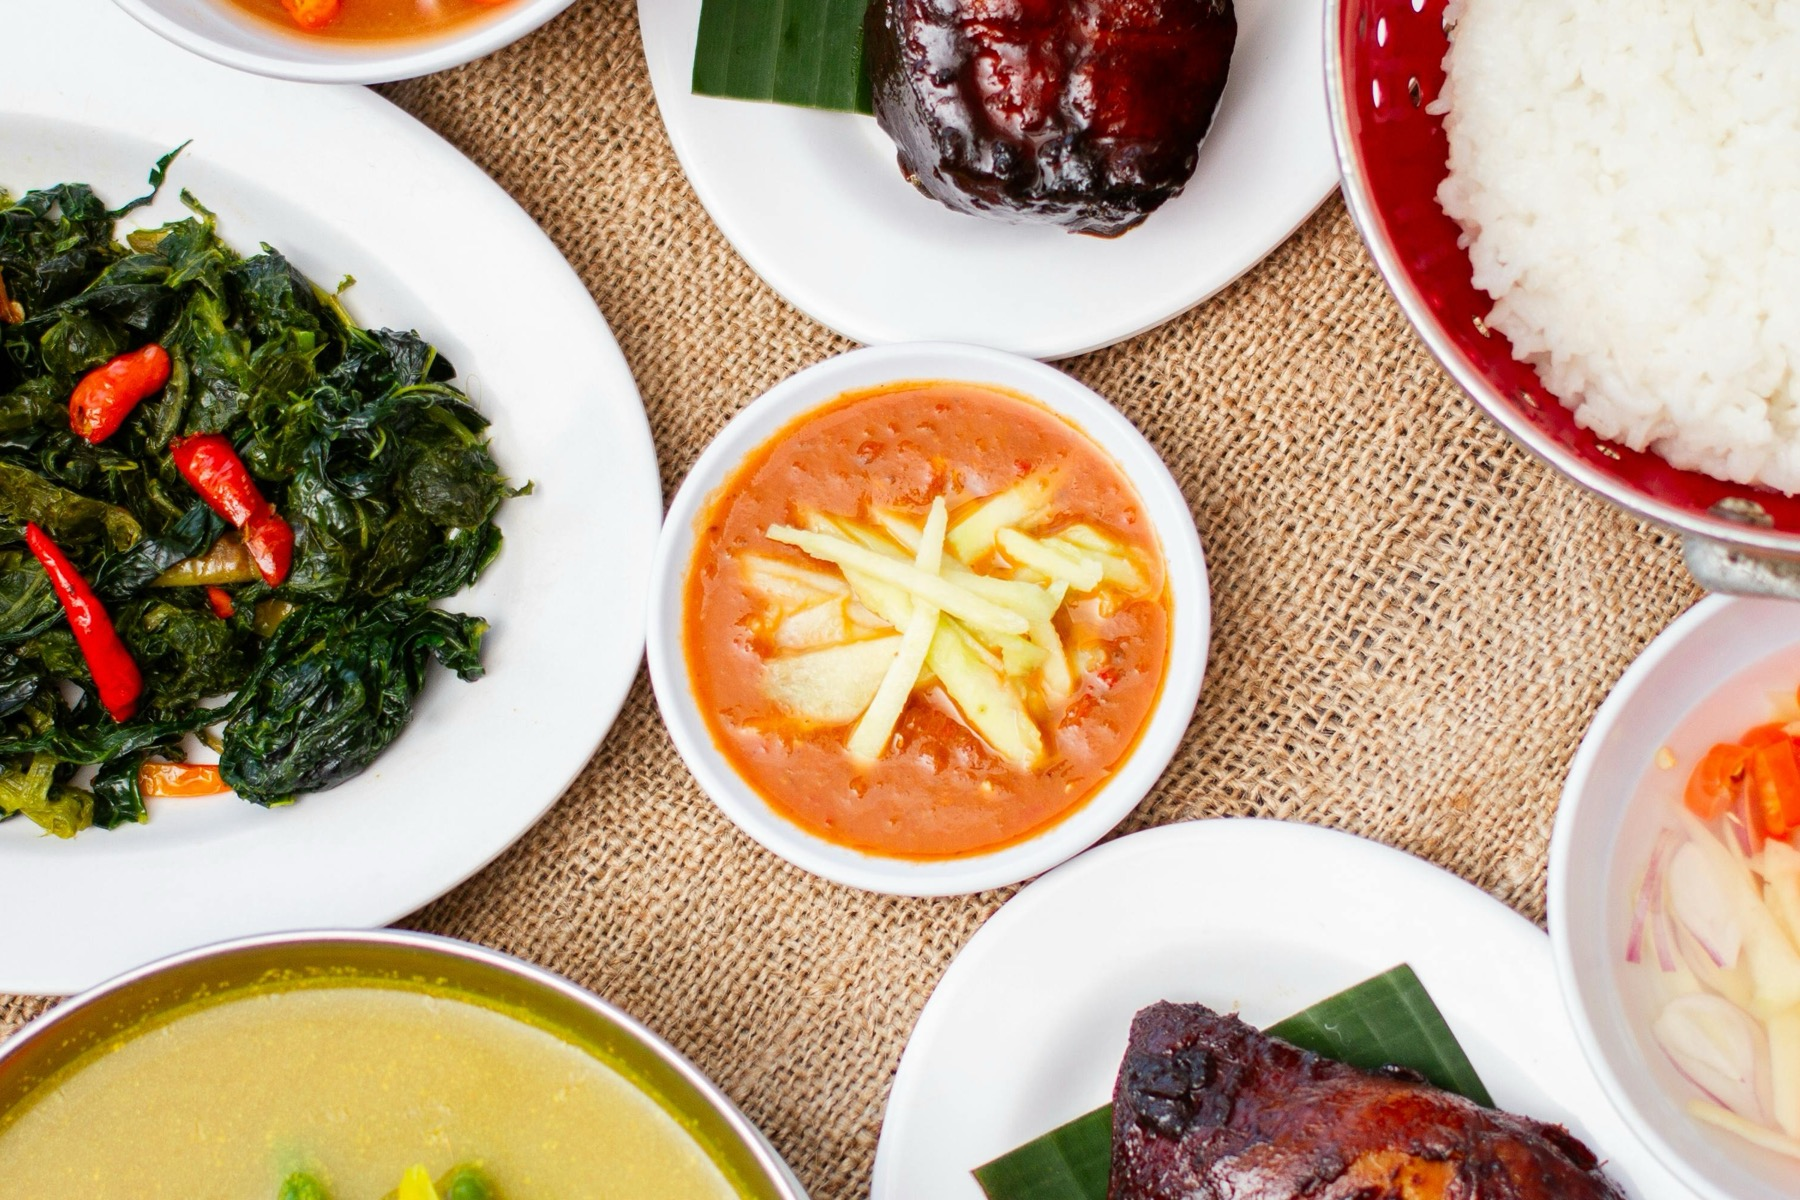
\includegraphics[width=0.25\textwidth]{figures/comparison_on_dataset_A/example_1/method_JEPA.jpg} \\

        
\includegraphics[width=0.25\textwidth]{figures/comparison_on_dataset_A/example_2/input_img.jpg} &

        % 
\includegraphics[width=0.25\textwidth]{figures/comparison_on_dataset_A/example_2/method_ResNet.jpg} &

        % 
\includegraphics[width=0.25\textwidth]{figures/comparison_on_dataset_A/example_2/method_Transformer.jpg} &

        % 
\includegraphics[width=0.25\textwidth]{figures/comparison_on_dataset_A/example_2/method_RNN.jpg} &

        
\includegraphics[width=0.25\textwidth]{figures/comparison_on_dataset_A/example_2/method_diffusion.jpg} &

        
\includegraphics[width=0.25\textwidth]{figures/comparison_on_dataset_A/example_2/method_mamba.jpg} &

        
\includegraphics[width=0.25\textwidth]{figures/comparison_on_dataset_A/example_2/method_JEPA.jpg} \\

        
\includegraphics[width=0.25\textwidth]{figures/comparison_on_dataset_A/example_5/input_img.jpg} &

        % 
\includegraphics[width=0.25\textwidth]{figures/comparison_on_dataset_A/example_4/method_ResNet.jpg} &

        % 
\includegraphics[width=0.25\textwidth]{figures/comparison_on_dataset_A/example_4/method_Transformer.jpg} &

        % 
\includegraphics[width=0.25\textwidth]{figures/comparison_on_dataset_A/example_4/method_RNN.jpg} &

        
\includegraphics[width=0.25\textwidth]{figures/comparison_on_dataset_A/example_4/method_diffusion.jpg} &

        
\includegraphics[width=0.25\textwidth]{figures/comparison_on_dataset_A/example_4/method_mamba.jpg} &

        
\includegraphics[width=0.25\textwidth]{figures/comparison_on_dataset_A/example_4/method_JEPA.jpg}

    \end{tabular}

    \caption{Additional qualitative comparison on Dataset A. Each row shows one example, and each column shows the input image or the result from a different method. 
    }

    \label{fig:comparison_dataset_A}

\end{figure*}

